%!TEX root = series of tubes.tex
\begin{figure*}
\centering
    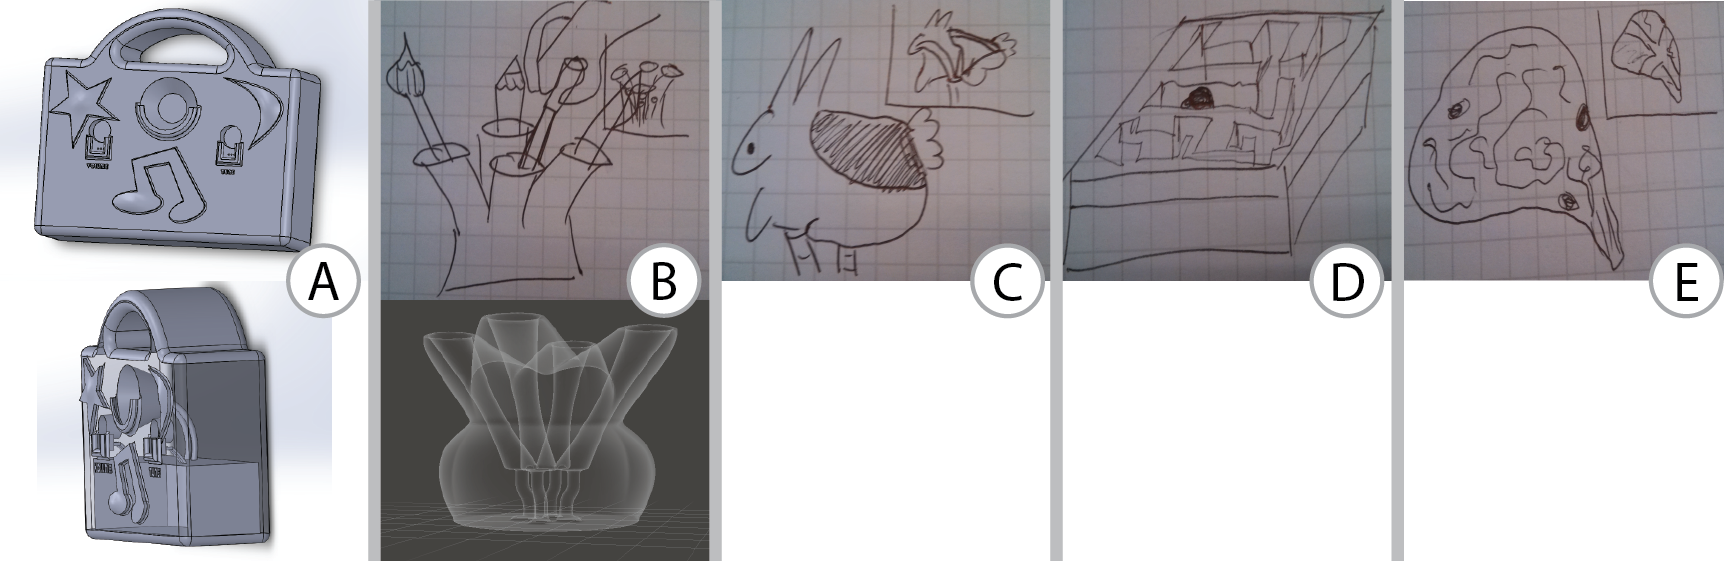
\includegraphics[width=7in]{figures/examples.png}
\caption{A series of example objects created using our system.  (a) is a touch-sensitive brain toy.  (b) is a rabbit which ``breathes'' using wind pipes we built.  (c) shows a portable radio.  (d) shows a presence-aware pen holder.  (e) is a maze game.}
\label{fig:examples}
\end{figure*}

\section{Example Objects}
\tovi{it might be intersting to relate our examples to existing HCI papers - in order we have: Touche, Dynamically Changeable Physical Buttons/PneUI, Midas, Suaron. I guess the maze doesnt really relate to anything.}
\tovi{UIST is someitmes cranky about providing enough details so other can reporduce the work. We might want to be more careful about providing specific part numbers of specifications.}
\bjoern{subsection headings need to be updated in light of the simplification and label changes in the design space.}
To evaluate and highlight our tool's capabilities, we fabricated a set of five prototype objects designed using \systemnamenospace.  \tovi{might want to specify the exact printer models we used here, and say we used multipel printers to show that are approach is printer independant.}
%All prototypes were fabricated in a single piece, unless described otherwise. \bjoern{2 of 5 will have been fabricated otherwise -  Radio, Neon sign - both in pieces.}

\subsection{Touch-sensitive Toys (open, liquid, star, terminals)}

To show how conductive fluids can be used for touch sensing, we created a set of touch-sensitive toys and a companion app that identifies the objects as well as touched parts of the objects (inspired by \cite{Harrison-acoustic}). The objects --- a brain and boat, in our example --- can be set on a base, upon which a speaker announces ``brain'' or ``boat''. Touching the brain model's front protrusion yields the announcement ``olfactory bulb''. The distinct touch points on each object are connected by an interior star topology, and touch sensing is performed via a single conductive connection to the base, using swept-frequency capacitive sensing~\cite{Sato-touche} (see Figure \ref{fig:toys}). %We built a smart base which can distinguish between the toys and also determine which toy is mounted:
Since each toy and each gesture has a distinct capacitive signature, we use a simple classifier trained to detect both toy and gesture based on profile.

The models we used for the toys were downloaded from the  Thingiverse website. We then used \systemnamenospace to create the desired internal pipes. All components were fabricated on a Makerbot, support-free.  After printing, we injected copper paint (CuPro-Cote) into the interior pipes using a craft syringe.  This paint requires approximately 2 days to fully dry in this configuration (3mm diameter tubes, maximum tube length 10cm).  Our smart base is powered by an Arduino Uno running open-source SFCS code\footnote{http://www.instructables.com/id/Touche-for-Arduino-Advanced-touch-sensing}. An advatnage of using this paint is that it also serves as an adhesive, so no soldering was required. \tovi{confirm}

\subsection{Breathing Bunny (semi-closed, gas, terminals)}

To demonstrate how gases can be used to both provide sensation to the user through openings and to deform a model internally, we created a rabbit with a pair of tubes that can simulate breathing (see Figure \ref{fig:breathe}).  When the rabbit inhales through its nose, its abdomen rises, and as it exhales its abdomen falls.  For this, we used a combination air/vacuum pump: one terminal creates a vacuum while the other creates positive pressure.  
The rabbit model was downloaded from the Thingiverse website. \tovi{confirm} We then used \systemnamenospace to add two pipes: one open pipe exiting at its mouth, and one semi-closed pipe capped at its abdomen.  We connected one pipe to each of our pump's terminals, and using a programmable power supply we mimic a rabbit's breathing pattern.  This example was printed on the Objet using a flexible material and its support material was flushed post-print.\tovi{give pump part number/details}

\subsection{Custom Radio (open, threadable, terminals)}
\tovi{stick with the strucutre - describe what it does, then describe modeling and fabrication (how it was built)}
A custom radio shows how pipes can be used to integrate electronic components into the user-facing surface of an object. The radio includes a power and volume dial, and LED which goes on when the radio is on, and a tuner dial. \tovi{confirm}. A Arduino Pro Micro microcontroller, Si4703 radio tuner, and  [x volt] power supply are embedded in the base of the radio. The sound is played through a single speaker. 

The radio was manually modelled in SolidWorks. We included slots on the 3D model matching the shape of the electronic components that were to be embedded. The model was then imported into \systemnamenospace, where we created a network of 8 individual open pipes (3 per potentiometer, 1 for the LED, 1 for the speaker) to connect the the comments to the base of the radio. We fabricated the radio itself on our Makerbot, support-free, but cut in two pieces to allow the Arduino and battery pack to be inserted. We then threaded the pipes with wires to connect the compoenents to the microcontroller at the base of the radio. 

%This design with 8 pipes (3 per potentiometer, 1 for the LED, 1 for the speaker) showed the limitations of our incremental routing strategy: since we voxelize and remesh for each pipe, surface detail is incrementally lost. The problem can be addressed by increasing the voxel resolution. At 512x512x512 voxels, surface geometry is not notably degraded. However, a single cut operation takes around 3 minutes \bjoern{on what hardware? mention earlier}, compared to near-instant performance on a $128^3$ voxel grid.  We fabricated the radio itself on our Makerbot, support-free but cut in two pieces to allow the Arduino and battery pack to be inserted. TOVI: Move to discussion if you want to keep this text.

\bjoern{I ran out of steam somewhere here...}
\tovi{relate this to sauron as well}
\subsection{Presence-aware Pen Holder (open, solid, ternimals)}
\bjoern{isn't this a threadable instead of a solid?} \bjoern{the model looks like the acutal pipes are really short and basically straight at the bottom of the model. This may raise the question if one couldn't just use the line sensors without any fiber optic cable in the middle.}
Our presence-aware pen holder can distinguish which tool or tools a user has picked up (see Figure \ref{fig:pens}).  Our pen holder uses a modification of the FlyEye technique described by Wimmer in \cite{Wimmer-flyeye} in which \bjoern{describe...}. 

The model was created/downloaded from [x]. We used \systemnamenospace to add four internal open pipes connecting each pen chamber to the based on the pen holder. This prototype was built by our Objet and support was flushed post-print.\bjoern{Incorrect. Looks like a Makerbot print.} \valkyrie{this whole paragraph is unclear}

Each pipe was then threaded with a fiber optic cable.  We use a single cable per pipe; our 6mm diameter fiber optic cables, in comparison to the fine tubes used in the original work , can send and receive through the same cable. \bjoern{is this because it has many strands?}  At the base of each tube is a QRE1113 line sensor digital breakout board, which has an integrated IR emitter and receiver.   When a pen is in its appointed place, the emitted infrared light is reflected off its bottom and travels back to the receiver, where it registers as bright.  

\subsection{Animated Neon Sign (return, threadable, path)}

\begin{figure}[h!]
\centering
    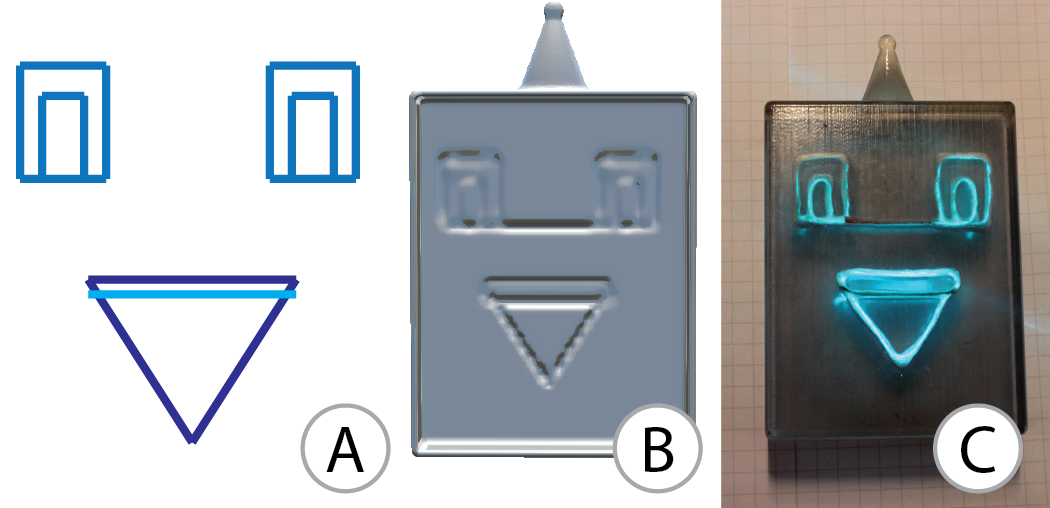
\includegraphics[width=3.4in]{figures/sign.png}
\caption{A two-state animated neon sign designed using our tool.  (a) shows the input SVG files, with the two states of the mouth drawn in different colors. \bjoern{it's hard to tell these colors apart!}  (b) shows the resultant mesh when we subtracted the generated tubes. \bjoern{hard to see what's going on here, too.} In (c), we show the fabricated sign.}
\label{fig:neon}
\end{figure}

Neon art is traditionally made from hand-formed glass tubes containing neon gas.  The tubes light up when a current is passed through them.  For this type of art, the path of the tubes is of crucial importance, as it determines how the sign will look.  We designed a custom neon robot head which can be animated to ``talk''.  
\tovi{in the system seciton do we ever discuss how entry and exit points are specified for path-constrained pipes?}
The geomertry of the model was imported into \systemnamenospace, which created the assocaited Pipes using its internal path routing tool. We then printed the model on the Objet using a transparent material. The model was printed in two halves, cutting through the plane of pipe path, to facilitate assembly. 

The pipes were threaded with electroluminescent wire which is lit in sequence to create an animation using an EL wire sequencer. Pipes enter and exit through the rear to hide the EL wire controls.  

\subsection{Maze (fully enclosed, particulate, tree, terminals + path)}

Our final example object is a maze game with a marble that can be navigated through a maze-like path, with exits on either side of the model. 

The maze is based on an SVG file we manually created and processed with our internal path routing tool.  The Maze was printed on the Objet using a transparent material. We created the maze in two halves that were fastened together via glue, to support the removal of support materials using a high-pressure water tool.  \bjoern{check - i think the latest maze is in fact done with our tool? Will need rewriting.}